\documentclass[10pt,twocolumn]{scrartcl}
\usepackage[a4paper,width=170mm,top=25mm,bottom=25mm,bindingoffset=3mm]{geometry}
\setlength{\parskip}{1em}
\usepackage[colorlinks=true, linkcolor=blue, citecolor=blue, urlcolor=blue]{hyperref}
\usepackage[numbers]{natbib}
\usepackage{hyperref}
\usepackage{lipsum}
\usepackage{graphicx} 
\usepackage{url} 
\usepackage{lipsum} 
\usepackage{float}
\usepackage{amsmath}
\usepackage{subcaption}
\usepackage{mwe}
\usepackage{multicol}
\usepackage{comment}

\renewenvironment{abstract}
 {\quotation\large\noindent\rule{\linewidth}{.5pt}\par\smallskip
  {\centering\bfseries\abstractname\par}\medskip}
 {\par\noindent\rule{\linewidth}{.5pt}\endquotation}

\begin{document}

\renewcommand{\refname}{References}

\twocolumn[
\begin{@twocolumnfalse}
	\title{ePATH Test Bench}
\author{Andreani Kalatha}
\maketitle

\begin{abstract}
Lorem ipsum dolor sit amet, consectetuer adipiscingelit. Ut purus elit, vestibulum ut, placerat ac, adipisc-ing vitae, felis. Curabitur dictum gravida mauris. Namarcu libero, nonummy eget, consectetuer id, vulputatea, magna.  Donec vehicula augue eu neque.  Pellen-tesque habitant morbi tristique senectus et netus etmalesuada fames ac turpis egestas. Mauris ut leo. Crasviverra metus rhoncus sem.  Nulla et lectus vestibu-lum urna fringilla ultrices. Phasellus eu tellus sit amettortor gravida placerat. Integer sapien est, iaculis in,pretium quis, viverra ac, nunc. Praesent eget sem velleo ultrices bibendum.  Aenean faucibus.  Morbi do-lor nulla, malesuada eu, pulvinar at, mollis ac, nulla.Curabitur auctor semper nulla. Donec varius orci egetrisus.  Duis nibh mi, congue eu, accumsan eleifend,sagittis quis, diam. Duis eget orci sit amet orci dignis-sim rutrum.
\end{abstract}
\end{@twocolumnfalse}]

\section{Introduction}
\subsection{Project Overview}
The purpose of this project is to check that the PCB board of ePATH functions properly. This would help ensure that it was properly manufactured by the factory and it will help smooth identification of faults during maintenance. The process must be automated and user-friendly to enable any technician without good knowledge of the electronics of ePATH perform this test. A


\begin{figure}[H]
          \centering
          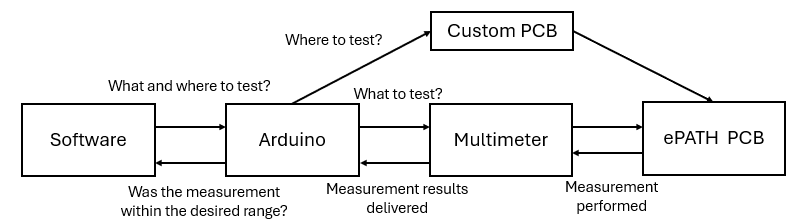
\includegraphics[width=1\linewidth]{img/General end goal diagram.png}
          \caption{Image 1}
          \label{fig:1}
    \end{figure}

\subsection{Main Objective}
The specific objectives of the project were: 
\begin{itemize}
\item 
\item To ...... 
\item To ...............
\end{itemize}

\subsection{Extra section}
\lipsum[1] 
\section{ePATH Test Bench}

\subsection{Multimeter connection}
It posed a challenge to establish the Computer-Arduino-Multimeter communication. Originally, the goal was to use the oscilloscope RIGOL MSO1104 Z but we couldn't find the drive needed to connect it to the computer. Eventually, we ended up using the multimeter Agilent 34401A 61/2 Digit Multimeter\cite{keysight34401A}. 

The most prominent difficulty was that the multimeter received commands but did not transmit anything back. For example, when sending a MEAS:VOLT:DC? command, the voltage was displayed on the multimeter screen but not sent to the computer. This was resolved after adjusting the MAX3232 connector. A 3.5kOhm pull-up resistor was utilized and connected as shown in \ref{MAX3232}.

\begin{figure}[H]
          \centering
          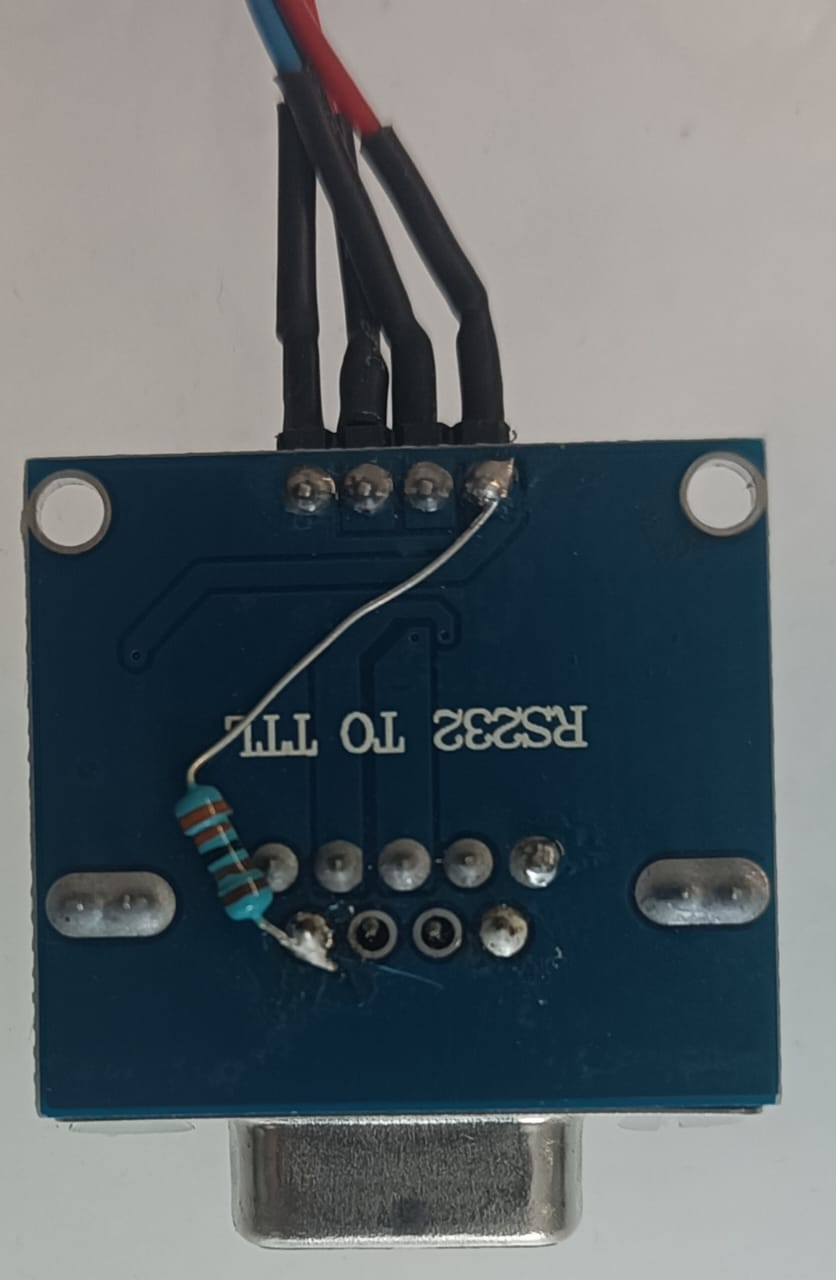
\includegraphics[angle=90, width=0.5\textwidth]{img/RS232_connector.jpeg}
          \caption{Picture of MAX3232 with 3.5kOhm pull-up resistor.}
          \label{MAX3232}
    \end{figure}

Some code that successfully enables communication between an Arduino DUE and the multimeter can be found in the Resources folder under the name Code that worked. This is useful to test initial communication with the multimeter. The connections of the Arduino DUE and the MAX3232 module are as shown in Figure \ref{MAX3232_Arduino}.

\begin{figure}[H]
          \centering
          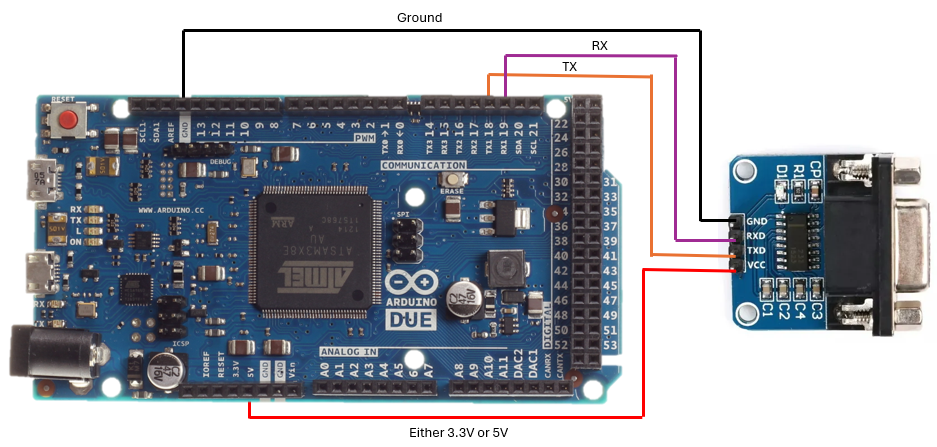
\includegraphics[width=1\linewidth]{img/MAX3232_connection.png}
          \caption{Electrical connection of Arduino DUE and MAX3232.}
          \label{MAX3232_Arduino}
    \end{figure}


\subsection{PCB version 1}
After some prototyping with a breadboard, the first version of the PCB was developed. It was given the name 'Automated DMM tester V1'. The purpose of this version is to test everything works smoothly and identify areas of improvement. 

A 16 channel MUX was chosen to direct the current of each ePATH pin to the multimeter so that the tests can be performed. A MUX was chosen over alternatives, such as shift registers with relays, for its simple wiring and fast operation \cite{tiMAX3232guide}. A 16 channeled one was chosen as there are 12 pins to be tested.

The kiCAD design of the PCB is stored in the resources folder under PCB attempt 1. When soldering the components on the board some alternations were made; instead of $330\,\Omega$ resistors, $1.6k\,\Omega$ resistors were used and instead of $10k\,\Omega$ resistors $4.6k\,\Omega$ resistors were used. The Arduino program used on it to test the functionality of the board is saved in the resources folder under PCB programming. 

In the schematic, the $330\,\Omega$ resistors were chosen since the forward voltage drop for white LEDs is approximately 2.4V and the desired current flow through them is about 10mA. Therefore:
\[
R = \frac{V}{I} = \frac{5\,\mathrm{V} - 2.4\,\mathrm{V}}{10\,\mathrm{mA}}=260\Omega
\]
Since $330\,\Omega$ is very close to the desired resistance and is a more readily available resistor value it was chosen for the schematic. In the end the $10k\,\Omega$ resistors used proved to work well.


There was a number of errors with this design:
\begin{itemize}
\item The footprint used for the banana socket is wrong. It only has a hole for the cental pin of the socket but not for the other 4 pins. This led to receiving an inquiry about it from the PCB manufacturers but this was easily resolved.
\item The orientation of the button footprint is incorrect-it should be rotated by 90 degrees. This issue was bypassed when making the button connection to the board but an awkward connection was produced.
\item When testing the PCB with the ePATH board it was discovered that upon trying to measure negative voltages the PCB stopped working. The PCB was tested and it was established that it can measure a minimum voltage of around -0.5V. Therefore, a different MUX capable of enabling negative voltage measurements should have been used.
\item The wiring of the Restart button is incorrect. It was not connected to the Arduino DUE pin 8 properly. This was corrected on the board by adding a wire according to the diagram in Figure \ref{button_wiring}.
\end{itemize}

\begin{figure}[H]
          \centering
          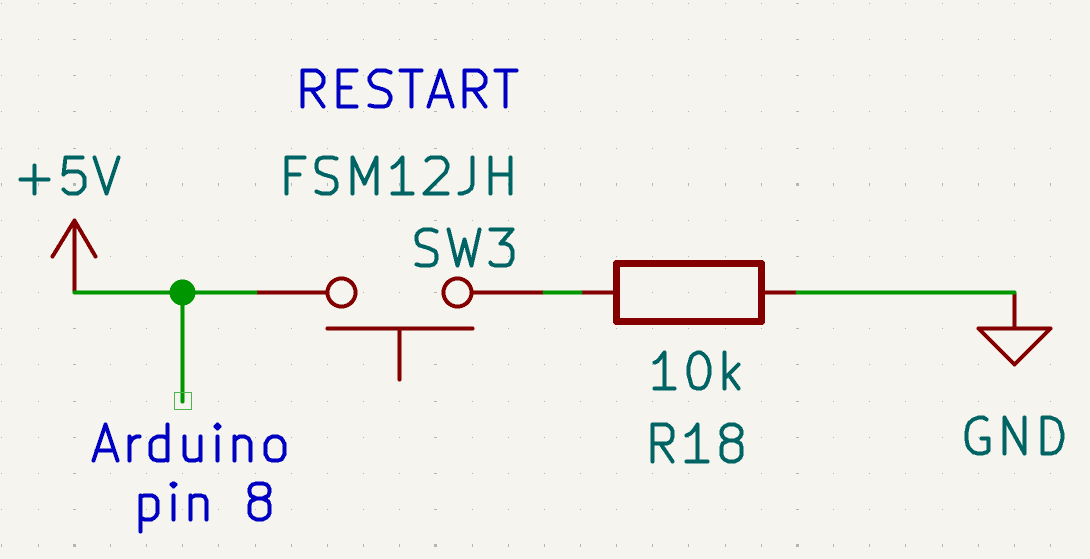
\includegraphics[width=1\linewidth]{img/button_wiring.png}
          \caption{Corrected electrical connection of RESTART button}
          \label{button_wiring}
    \end{figure}



\subsection{PCB version 2}
The second version of the PCB was given the name 'Automated DMM tester V2-July 2025'. The purpose of this version is to perform some tests with ePATH. The improvements made for this version include:
\begin{itemize}
\item To facilitate the connection between the test points on ePATH with the PCB, a D-sub connector was implemented.
\item The PN532 module capable of obtaining the RFID tag of the ePATH board \cite{pn532manual} was implemented.
\item Instead of using a multiplexer, shift registers and relays were used. That's because relays are optically isolated which minimizes noise. 
\item Since the number of electrical components being controlled by the Arduino increased in this PCB iteration, an external voltage source was required; the PCB could no longer be powered by the Arduino. For that reason a 5V voltage regular was implemented.
\item Since the ePATH board has 2 grounds a control system to switch between them was implemented.
\item A digital potentiometer was implemented to produce the resistances needed for some of the ePATH board tests. In order to confirm that the potentiometer produced the correct resistances a port was implemented across it.
\end{itemize}

The kiCAD design of the PCB is stored in the resources folder under PCB attempt 2. To enhance my understanding of shift register operation I wired up the relays and shift registers in TinkerCad and ran some simulations. The simulation is stored in the resources folder under Shift registers sim.



\subsection{GUI}
A user friendly GUI has been developed to facilitate the testing of the ePATH PCB. The code for the GUI is on the ePATH-Test-Bench project of the company's GitHub \href{https://github.com/pathfinder-medical/ePATH-Test-Bench}{here}.

The key functionalities of the GUI include:
\begin{itemize}
\item Run button; Starts the testing cycle.
\item Clear button; Deletes all testing results for re-tests.
\item Save button; Saves a pdf file with the table of results.
\item Get button; Gets the RFID of the ePATH board.
\end{itemize}

\section{Extra projects}

Some additional small projects were undertaken in parallel to ePATH Test Bench project.

\subsection{Electrical display switching}
To test the functionality of the device during animal studies, it was proposed that the Target and Crossing catheters are connected to three different ePATH displays. To make the change between displays as easy as possible without requiring the removal of the catheters from the animal's body a switching mechanism is required. While the mechanical switching between the displays with switches was already explored, an electrical decision was required. Some electrical components that would enable the switching were explored as follows.

\subsubsection{Background}
Firstly, the idea of using solid state relays(SSRs) was explored \cite{ssr_rfwireless}. A large advantage of using this is that SSRs are optically isolated. Therefore, the input and output are physically isolated when the current is below a certain level which enhances precision by minimizing noise. This will be very useful in this system as interferences from the different displays will have no effect on how the system behaves. Other advantages include their ability to work with both DC and AC signals, their silent operation and low power consumption. A problem when working with SSRs is that they break easily. 

Secondly, transistors were considered as an alternative switching method as they are widely used as switches \cite{transistor_switch}.  They offer a wide range of advantages such as current control, controlling the exact current that would enter the ePATH display, and offer quick switching. Transistors can be arranged in Darlington or Sziklai configurations which increases the input impedance further. There is a wide variety of transistors for different operating conditions thus choosing the appropriate transistor involves more calculations. A big disadvantage is that the inputs and outputs are not isolated so even if the transistor if off there might be some leakage current that interferes with the operation of the system.

Multiplexers can also function as switches. For example, the SN74CBT16214CDLR \cite{sn74cbt_datasheet} provides twelve independent 3:1 MUX channels that could be used for this purpose. However, once again there is a direct physical connection between the inputs and outputs. This could pose problems if the circuit is not powered or if the MUX malfunctions, potentially allowing unintended signal paths. Controlling the MUX with an Arduino would also increase the system’s complexity. Furthermore, there are limitations on which ports can be used simultaneously, which could restrict potential future expansions of the project.

Tri-state buffers were also considered to be used as switches. They enable or disable the connection between input and output via changes in impedance \cite{digital_buffer}. However, they were quickly ruled out upon determining that their output is limited to only three states: logic high (1), logic low (0), or high impedance (Z). As a result, they cannot transmit complex analogue signals, which are the type of signals involved in our application. Another component that was quickly rejected was the silicon-controlled rectifier (SCR) \cite{scr_switch}. The main drawback is the difficulty of turning off a conducting SCR, which requires specialized commutation circuits to force the switch open. Additionally, SCRs can unintentionally turn on due to a high rate of voltage change (dv/dt) at the source which might occur due to electrical interference. It should be noted however that one advantage of the SCR, compared to a transistor, is that it operates strictly in binary states: either fully on or fully off, with no active region of operation.

For the reasons outlined above, particularly the significant advantage of opto-isolation, relays were selected to implement the electrical switches. These relays will be controlled by shift registers, which are themselves managed by an Arduino. Shift registers were chosen as they are relatively easy to control and have flexible functionality allowing many pins to be on simultaneously.

\subsubsection{Design proposition}
Design one:

The crossing catheter has 4 connecting wires and the target catheter 2. Therefore, 6 connections per display need to be switched on and off. Since there are 3 displays, this is an overall of 18 connections that need to be controlled. Therefore, 18 Single Pole Single Throw(SPST) relays would need to be used, or 9 Single Pole Double Throw relays like ASSR-1420-302E \cite{assr_datasheet} or 6 Single Pole Thee Throw relays like FMSW6362 \cite{relay_switch. These can be controlled by 8-bit shift registers like SN74AHCT595PWR \cite{shift_register}. The block diagram below shows the connection between a particular pin on a catheter and it’s corresponding connecting point with the displays when using SPST relays. Another 15 such connections would need to be wired.

\begin{figure}[H]
          \centering
          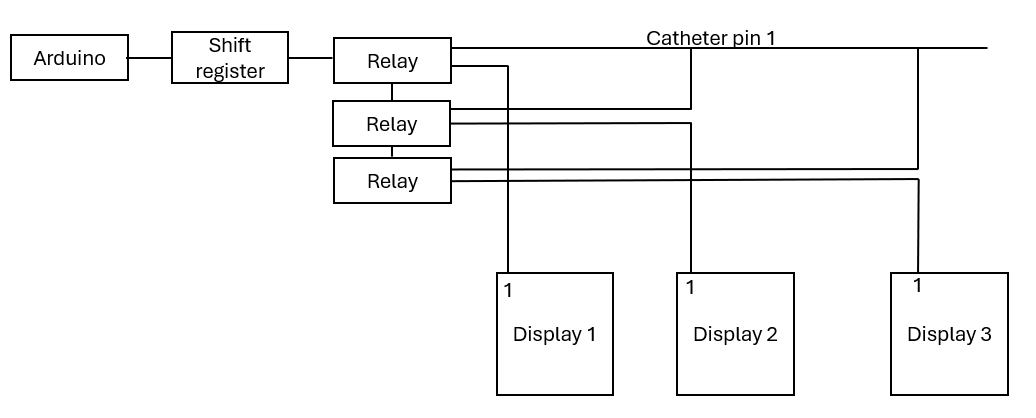
\includegraphics[width=1\linewidth]{img/Design1.png}
          \caption{Block diagram of first design proposition}
          \label{button_wiring}
    \end{figure}
    
A disadvantage of this design is the large amount of relays and thus wiring needed.

Design two:

In order to minimize the number of relays and connections needed, an alternative solution is to connect the inputs of the 3 displays and selectively turn on the display we want to use. This would mean that data is sent to all displays but only the display that is turned on is processing it.
To turn on and off the appropriate display, relays can be used. Each display is powered by 2 wires; the ground and the voltage wire. The ground connection of all the displays can be connected. The voltage wire of each display can be switched on and off using 3 SPST relays controlled by a shift register.  The block diagram of such a connection is shown below.
\begin{figure}[H]
          \centering
          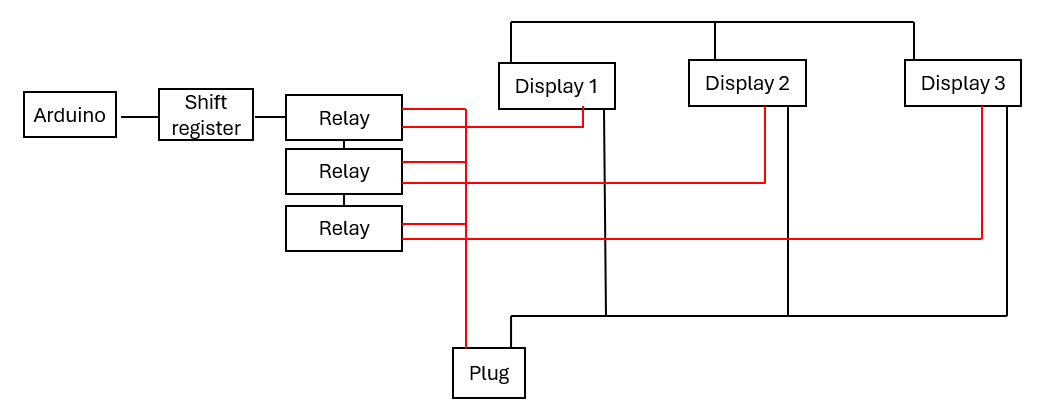
\includegraphics[width=1\linewidth]{img/Design2.png}
          \caption{Block diagram of second design proposition}
          \label{button_wiring}
    \end{figure}
An issue with this wiring method is that when sending commands to a display that is turned off some interference can be created which will affect its functionality when it’s turned on. Another issue is that the displays take some time to turn on thus this method would be slower. Therefore, this is deemed a worse design than Design 1.


\subsubsection{Conclusion}
In conclusion, to electrically switch the catheter connections between the three ePATH displays, a combination of relays and shift registers was determined to be the most effective solution. Among the configurations considered, Design 1 was found to be the most suitable for implementing the system with minimal interference.





\subsection{Text file saving}
Data printed in the Serial monitor of Arduino IDE can easily be lost and is difficult to work with. To make data acquisition and handling easier, a simple GUI was developed that captures the printed data and saves it in a .txt file. The GUI consists of a:
\begin{itemize}
\item A list-box that displays the information printed on the Serial monitor. 
\item A save button that saves the data in a text file at the desired directory.
\item A clear button that deletes data in case they were corrupted.
\item A information button that displays an information window that explains the GUI's functionalities.
\end{itemize}

The python code used to develop this GUI is in the resources folder of this document under the name Save text files. An Arduino code that prints out the numbers from 1-100 is also provided for demonstrative purposes.

\begin{table*}[ht]
    \centering
    \begin{tabular}{p{0.25\linewidth}p{0.25\linewidth}p{0.25\linewidth}}
    \hline
    column 1 & column 2 & column 3\\
    \hline
    1 & 2 & 3\\
    1 & 2 & 3\\
    1 & 2 & 3\\
    1 & 2 & 3\\
    \hline
    \end{tabular}
    \caption{Another random table}
    \label{tab:2}
\end{table*}
\noindent Another type of table for your results below.

\subsection{Subtopic 2}
\lipsum[1]

\noindent Another figure grid example: (on next page)

\begin{figure*}[ht]
\begin{multicols}{2}
        \centering
        \begin{subfigure}[b]{0.475\textwidth}
            \centering
            
\includegraphics[width=\textwidth]{img/bioeng.jpg}
            \caption{Part 1}    
        \end{subfigure}
        \hfill
        \begin{subfigure}[b]{0.475\textwidth}  
            \centering 
            
\includegraphics[width=\textwidth]{img/bioeng.jpg}
            \caption{Part 2}    
        \end{subfigure}
        \vskip\baselineskip
        \begin{subfigure}[b]{0.475\textwidth}   
            \centering 
            
\includegraphics[width=\textwidth]{img/bioeng.jpg}
            \caption{Part 3}  
        \end{subfigure}
        \hfill
        \begin{subfigure}[b]{0.475\textwidth}   
            \centering 
            
\includegraphics[width=\textwidth]{img/bioeng.jpg}
            \caption{Part 4}    
        \end{subfigure}
        \label{fig:mean and std of nets}
        \end{multicols}
        \caption {A figure grid} 
        \label{fig:3}
    \end{figure*}

\section{Discussion}

\subsection{Subtopic}
\lipsum[1]
\subsubsection{Part 1}
\lipsum[1]
\section{Conclusion}

\subsection{Summary}
\lipsum[2]

\noindent If you want to list some of your closing points here is an example:
Our concluding points are...
\begin{enumerate}
  \item Concluding point .....
  \item Concluding point.....
  \item Concluding point.....
\end{enumerate}


\subsection{Future Work}

\noindent To close this template, let's look at referencing. Make sure you have a references.bib files (check the example in this template) and then cite as follows:

\noindent Here I am mentioning something linked to my first reference. \cite{Barbero2012} 

\noindent Here I am mentioning something linked to my second reference. \cite{Farina2020}

\noindent Here I am mentioning something linked to my third reference. \cite{Saitou2000}

\noindent Make sure to check the latex documentation to reference different types of resources e.g. books, general communication, conference poster etc. in the correct way.

\newpage

\section{Appendix}

\noindent Add supplementary project information here. DON'T use as a workaround for the word count!!!
\bibliographystyle{plain}
\bibliography{references}

\end{document}